% Provenance (never printed): cycle 4 SVT, "La planete Terre, l'environnement
% et l'action humaine": natural risks, hazard and vulnerability, prevention
% and protection; see sources/book1/PROVENANCE.md. Book 1, grade 9, chapter 2.
% Vocabulary guard: owns risk, vulnerability, prevention, hazard map.
% Natural hazard and natural disaster, the warning colours and the safety
% rules are g5's (natural-hazards); the warning signs of an eruption and the
% Pinatubo story are g7's (volcanoes); seismometer, tsunami and "scientists
% cannot predict earthquakes" are g7's (earthquakes); flood and floodplain
% are g5's (water-shapes-the-land); weather forecast is g8's. Lahars are
% called mudflows (as in g7). "Normal fault" is Book 2's: here "a fault".
\chapter{Hidup Bersama Risiko Alam}\label{ch:g9:natural-risks}

Larut malam pada 13~November 1985, sebagian besar penduduk Armero, sebuah
kota di Kolombia, sudah tidur. \omterm{def:g5:natural-hazards:storm}{Badai} menyembunyikan \omterm{def:g4:volcanoes-earthquakes-first-look:volcano}{gunung api} Nevado del
Ruiz yang puncaknya bersalju, \qty{45}{km} jauhnya, dan tak seorang pun di
kota itu melihatnya meletus. \omterm{def:g3:stones-pebbles-sand:rock}{Batuan} panas mencairkan sebagian esnya, dan
air itu, bercampur dengan abu dan \omterm{def:g3:stones-pebbles-sand:rock}{batuan}, menerjang turun menyusuri
\omterm{def:g1:landscapes-around-us:landform}{lembah-lembah} sebagai aliran lumpur. Sekitar dua jam kemudian, aliran
lumpur itu keluar dari \omterm{def:g1:landscapes-around-us:landform}{lembah} \omterm{def:g1:landscapes-around-us:water}{Sungai} Lagunillas, langsung masuk ke kota:
sekitar \num{23000} orang, sebagian besar penduduk kota, tewas. Dua jam
sebenarnya cukup untuk berjalan kaki ke tempat yang lebih tinggi.
Penduduk Armero tidak diberi tahu.
% ledger: usgs:armero

\begin{omfigure}
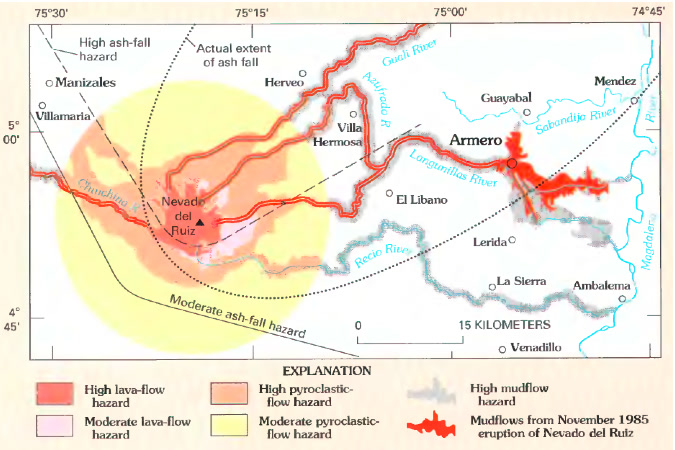
\includegraphics[width=0.86\linewidth]{images/book1/g9-ruiz-hazard-map.jpg}

{\small \omterm{def:g9:natural-risks:hazard-map}{Peta bahaya} Nevado del Ruiz. Versi pertamanya, yang digambar oleh
para ahli geologi Kolombia, sudah beredar satu bulan sebelum \omterm{def:g4:volcanoes-earthquakes-first-look:eruption}{letusan} dan
sudah menunjukkan bahaya aliran lumpur di \omterm{def:g1:landscapes-around-us:landform}{lembah} Armero. Versi ini, yang
digambar ulang setelah bencana, menambahkan dengan warna merah terang
aliran lumpur yang benar-benar datang pada bulan November 1985 (lingkaran
berarsir di sekeliling \omterm{def:g4:volcanoes-earthquakes-first-look:volcano}{gunung api} itu berjari-jari sekitar
\qty{20}{km}). Dari T.~L.~Wright dan T.~C.~Pierson, USGS Circular 1073, 1992
(domain publik, melalui Wikimedia Commons).}
% ledger: usgs:ruiz-map, commons:ruiz-map
\label{fig:g9:natural-risks:ruiz}
\end{omfigure}

Enam tahun kemudian, di Gunung Pinatubo di Filipina, \omterm{def:g4:volcanoes-earthquakes-first-look:volcano}{gunung api} itu
diawasi, peringatan datang tepat waktu, dan penduduk pergi mengungsi
(\cref{ch:g7:volcanoes}). Keduanya \omterm{def:g4:volcanoes-earthquakes-first-look:volcano}{gunung api} yang meletus secara
eksplosif, dengan penduduk yang tinggal di jalur aliran lumpurnya. Yang
berbeda adalah apa yang diketahui orang, dan apa yang mereka lakukan
dengan pengetahuan itu. Bab ini membahas perbedaan tersebut.
% ledger: usgs:armero (Pinatubo 1991 averted a disaster like Armero), usgs:pinatubo-1991

\begin{recall}
\emph{\omterm{def:g5:natural-hazards:hazard}{Bahaya alam}} adalah peristiwa alam yang dapat mencelakai manusia;
bahaya itu menjadi \emph{\omterm{def:g5:natural-hazards:disaster}{bencana alam}} ketika melanda tempat tinggal
manusia dan menimbulkan kerugian yang besar (\cref{ch:g5:natural-hazards}).
\omterm{def:g1:landscapes-around-us:water}{Sungai} yang meluap menggenangi \omterm{def:g5:water-shapes-the-land:flood}{dataran banjirnya}
(\cref{ch:g5:water-shapes-the-land}). \omterm{def:g4:volcanoes-earthquakes-first-look:volcano}{Gunung api} sering memberikan
tanda-tanda peringatan sebelum \omterm{def:g4:volcanoes-earthquakes-first-look:eruption}{letusan} besar: gempa-gempa kecil, lereng
yang menggembung, gas (\cref{ch:g7:volcanoes}). Para ilmuwan tidak dapat
meramalkan \omterm{def:g4:volcanoes-earthquakes-first-look:earthquake}{gempa bumi}; \omterm{def:g7:earthquakes:seismometer}{seismometer} merekamnya, dan \omterm{def:g4:volcanoes-earthquakes-first-look:earthquake}{gempa bumi} di bawah \omterm{def:g2:water-on-earth:ocean}{laut}
dapat memicu \omterm{def:g7:earthquakes:tsunami}{tsunami} (\cref{ch:g7:earthquakes}). \omterm{def:g8:fronts-and-weather-maps:forecast}{Prakiraan cuaca}
menyatakan \omterm{def:g1:watching-the-weather:weather}{cuaca} yang akan terjadi dalam beberapa hari mendatang
(\cref{ch:g8:fronts-and-weather-maps}).
\end{recall}

\section{Bahaya, kerentanan, dan risiko}

\omterm{def:g4:volcanoes-earthquakes-first-look:earthquake}{Gempa bumi} yang sama tidak menimbulkan kerugian yang sama di mana-mana. Di
bawah \omterm{def:g5:weather-and-climate:desert}{gurun} yang kosong, gempa itu tidak mencelakai siapa pun. Di bawah
kota dengan bangunan-bangunan yang kokoh yang penduduknya tahu apa yang
harus dilakukan, gempa itu mengguncang, menakutkan, dan memecahkan kaca
jendela. Di bawah kota dengan rumah-rumah yang berat dan dibangun dengan
buruk, gempa itu dapat merobohkan rumah-rumah itu menimpa orang-orang di
dalamnya. Bahayanya sama; yang berubah adalah seberapa mudah tempat itu
dapat dicelakai.

\begin{definition}[Kerentanan]\label{def:g9:natural-risks:vulnerability}
Yang disebut \emph{kerentanan}\index{kerentanan} suatu tempat adalah
seberapa mudah penduduknya, bangunan-bangunannya, dan barang-barang yang
mereka perlukan dapat dicelakai oleh suatu \omterm{def:g5:natural-hazards:hazard}{bahaya alam}. Rumah di \omterm{def:g5:water-shapes-the-land:flood}{dataran
banjir}, bangunan yang lemah, tidak adanya peringatan, dan tidak adanya
rencana membuat suatu tempat rentan.
\end{definition}

\begin{definition}[Risiko]\label{def:g9:natural-risks:risk}
Yang disebut \emph{risiko}\index{risiko} yang dihadapi suatu tempat dari
suatu \omterm{def:g5:natural-hazards:hazard}{bahaya alam} adalah ancaman kerugian bagi penduduknya dan harta
bendanya. Risiko bergantung pada bahayanya, yaitu seberapa kuat dan
seberapa sering bahaya itu terjadi, sekaligus pada \omterm{def:g9:natural-risks:vulnerability}{kerentanan} tempat itu:
di tempat yang tidak ada bahayanya, atau tidak ada yang dapat dicelakai,
tidak ada risiko.
\end{definition}

\begin{omfigure}
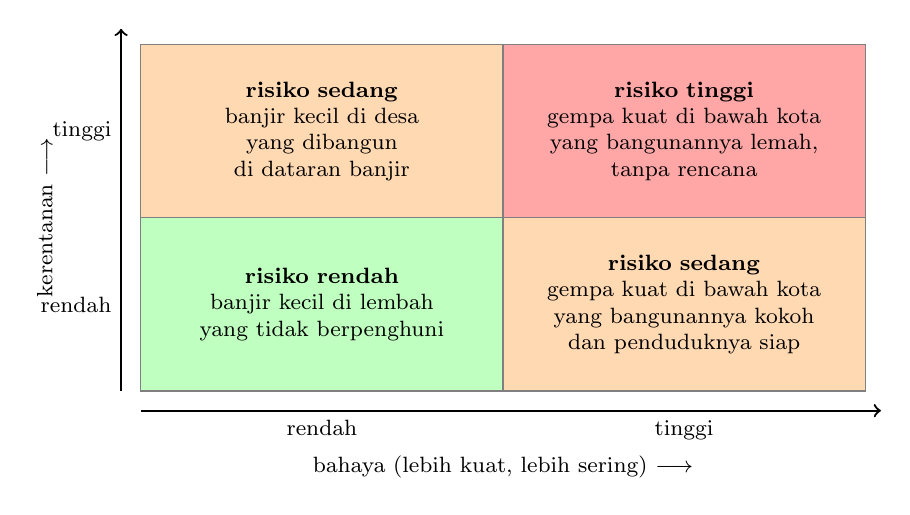
\begin{tikzpicture}[x=1cm, y=1cm, font=\footnotesize,
    cell/.style={minimum width=4.6cm, minimum height=2.2cm, align=center, draw=black!50, text width=4.2cm}]
  \node[cell, fill=green!25] at (2.3,1.1) {\textbf{risiko rendah}\\ banjir kecil di lembah\\ yang tidak berpenghuni};
  \node[cell, fill=orange!30] at (6.9,1.1) {\textbf{risiko sedang}\\ gempa kuat di bawah kota\\ yang bangunannya kokoh\\ dan penduduknya siap};
  \node[cell, fill=orange!30] at (2.3,3.3) {\textbf{risiko sedang}\\ banjir kecil di desa\\ yang dibangun di dataran banjir};
  \node[cell, fill=red!35] at (6.9,3.3) {\textbf{risiko tinggi}\\ gempa kuat di bawah kota\\ yang bangunannya lemah,\\ tanpa rencana};
  \draw[->, thick] (0,-0.25) -- (9.4,-0.25);
  \draw[->, thick] (-0.25,0) -- (-0.25,4.6);
  \node[anchor=north] at (4.6,-0.7) {bahaya (lebih kuat, lebih sering) $\longrightarrow$};
  \node[rotate=90, anchor=south] at (-1.0,2.2) {kerentanan $\longrightarrow$};
  \node[below] at (2.3,-0.25) {rendah};
  \node[below] at (6.9,-0.25) {tinggi};
  \node[left] at (-0.25,1.1) {rendah};
  \node[left] at (-0.25,3.3) {tinggi};
\end{tikzpicture}

{\small Kisi \omterm{def:g9:natural-risks:risk}{risiko} (sketsa). \omterm{def:g9:natural-risks:risk}{Risiko} bertambah besar bersama bahaya dan
bersama \omterm{def:g9:natural-risks:vulnerability}{kerentanan}. Memindahkan kota jarang mungkin dilakukan, dan bahaya
tidak dapat dimatikan; tetapi \omterm{def:g9:natural-risks:vulnerability}{kerentanannya} dapat diturunkan, sehingga
kota itu bergeser ke bawah pada kisi.}
\label{fig:g9:natural-risks:grid}
\end{omfigure}

Armero adalah tempat dengan bahaya yang tinggi: \omterm{def:g4:volcanoes-earthquakes-first-look:volcano}{gunung api} bersalju yang
telah bangkit setahun sebelumnya, dan kota yang dibangun di atas endapan
aliran lumpur lama, di mulut \omterm{def:g1:landscapes-around-us:landform}{lembah} yang dahulu pernah dilalui aliran
lumpur. Armero juga sangat rentan: para ilmuwan kekurangan peralatan dan
dukungan, keterangan yang diberikan kepada pihak berwenang sering kali
samar, dan tidak ada rencana evakuasi maupun cara cepat untuk
memperingatkan kota itu.
% ledger: usgs:armero

\section{Prakiraan dan pencegahan}

Sebagian bahaya dapat terlihat kedatangannya. \omterm{def:g5:natural-hazards:storm}{Badai} dapat diprakirakan
beberapa hari sebelumnya (\cref{ch:g8:fronts-and-weather-maps}); \omterm{def:g5:water-shapes-the-land:flood}{banjir}
setelah \omterm{def:g4:clouds-rain-snow:precipitation}{hujan} lebat, beberapa jam sampai beberapa hari sebelumnya; \omterm{def:g4:volcanoes-earthquakes-first-look:eruption}{letusan}
besar sering kali memberi tanda beberapa hari sampai beberapa minggu
sebelumnya, walaupun tidak selalu. \omterm{def:g7:earthquakes:tsunami}{Tsunami} menyeberangi \omterm{def:g2:water-on-earth:ocean}{samudra} dalam
hitungan jam, sehingga peringatan dapat mencapai pantai yang jauh lebih
dahulu daripada \omterm{def:g7:earthquakes:tsunami}{tsunami} itu. Sebaliknya, \omterm{def:g4:volcanoes-earthquakes-first-look:earthquake}{gempa bumi} tidak dapat
diramalkan: para ilmuwan dapat mengatakan \omterm{def:g7:earthquakes:fault}{sesar} mana yang suatu hari akan
patah lagi, tetapi tidak pernah harinya.
% ledger: nws:tsunami-speed, usgs:eq-basics, usgs:pinatubo-1991

Prakiraan, sebaik apa pun, hanya berguna jika sesuatu dilakukan sebelum
bahaya itu melanda. Sebagian besar pekerjaan itu dilakukan jauh sebelum
ada peringatan.

\begin{definition}[Pencegahan]\label{def:g9:natural-risks:prevention}
Yang disebut \emph{pencegahan}\index{pencegahan} adalah segala sesuatu yang
dilakukan sebelum \omterm{def:g5:natural-hazards:hazard}{bahaya alam} melanda untuk menurunkan \omterm{def:g9:natural-risks:risk}{risiko}: mengetahui
di mana bahaya itu dapat melanda, membangun di tempat yang aman dan dengan
cara yang aman, mengawasi bahayanya, memperingatkan penduduk, dan
mempersiapkan mereka.
\end{definition}

\omterm{def:g9:natural-risks:prevention}{Pencegahan} bekerja pada kedua sisi kisi \omterm{def:g9:natural-risks:risk}{risiko}. Mengawasi \omterm{def:g4:volcanoes-earthquakes-first-look:volcano}{gunung api} atau
\omterm{def:g1:landscapes-around-us:water}{sungai} tidak membuatnya kurang berbahaya, tetapi memberikan waktu untuk
bertindak. Membangun jauh dari \omterm{def:g5:water-shapes-the-land:flood}{dataran banjir}, membangun rumah yang kokoh,
merencanakan jalur ke tempat yang lebih tinggi dan melatihnya, semuanya
menurunkan \omterm{def:g9:natural-risks:vulnerability}{kerentanan}.

\begin{omfigure}
\begin{minipage}[c]{0.44\linewidth}\centering
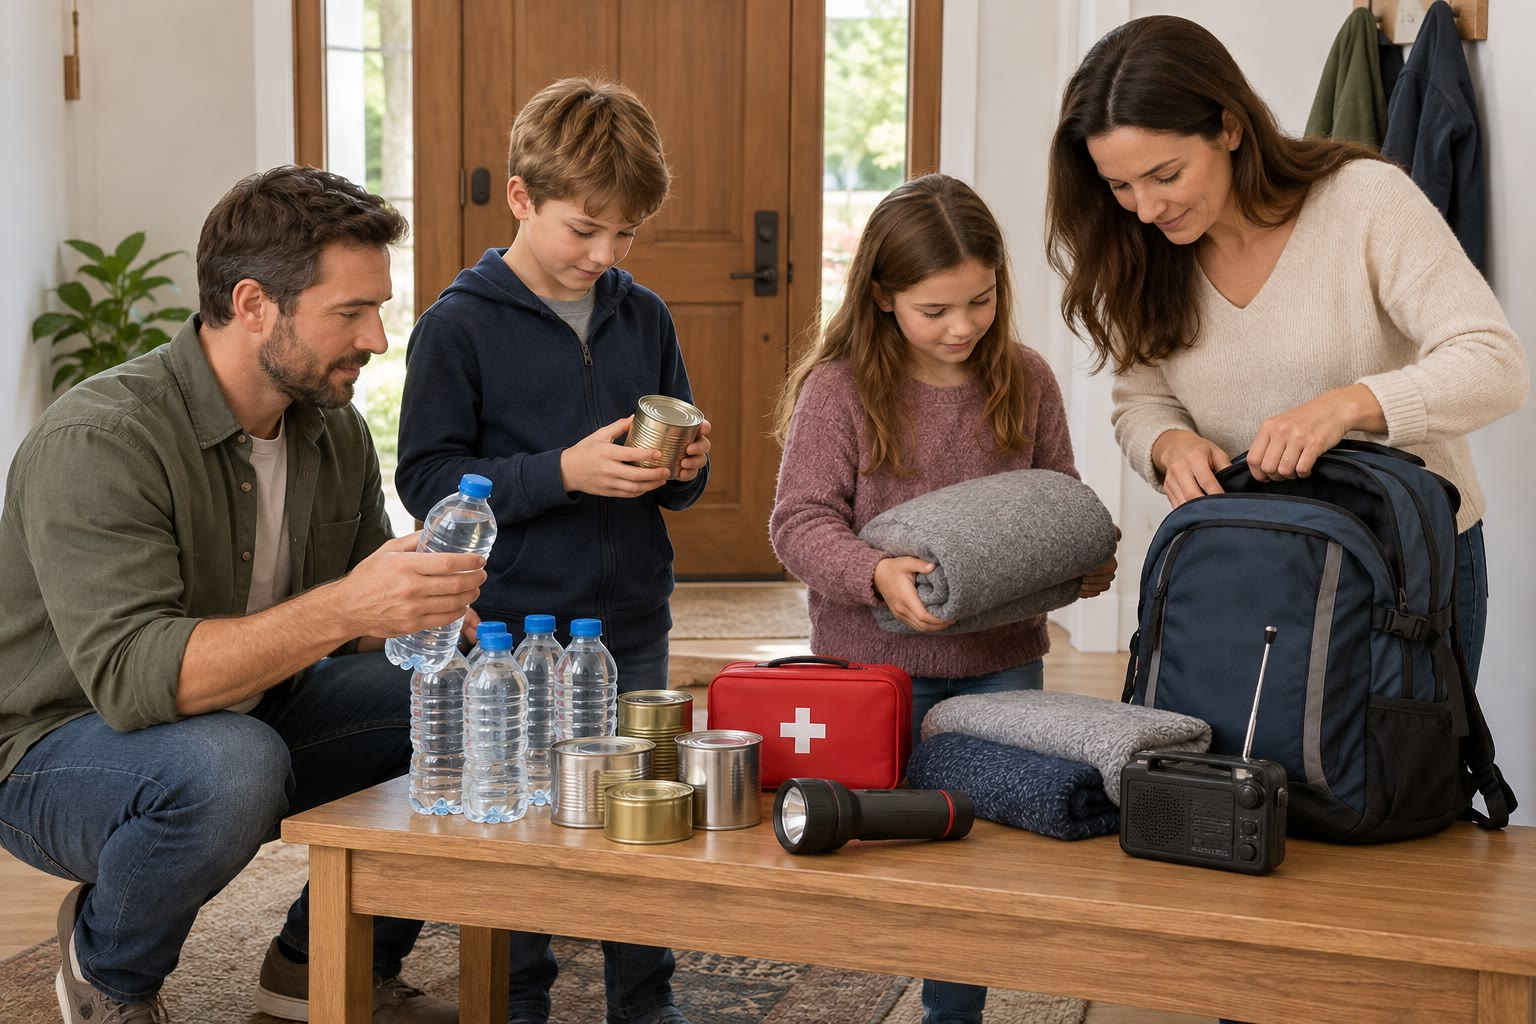
\includegraphics[width=\linewidth]{images/book1/ai/g9-emergency-kit.jpg}
\end{minipage}\hfill
\begin{minipage}[c]{0.52\linewidth}\raggedright
{\small Bersiap siaga: sebuah keluarga memeriksa tas siaga bencananya,
yang disimpan di dekat pintu, siap dibawa jika mereka harus pergi dengan
cepat: air dan makanan yang tahan beberapa hari, senter, radio yang dapat
bekerja tanpa listrik PLN, baterai cadangan, kotak P3K, dan selimut hangat
(ilustrasi AI dari suatu adegan umum).}
\end{minipage}
% ledger: ready:kit
\label{fig:g9:natural-risks:kit}
\end{omfigure}

\section{Mengawasi gunung api dan sesar}

Observatorium \omterm{def:g4:volcanoes-earthquakes-first-look:volcano}{gunung api} mengawasi tanda-tanda peringatan dari
\cref{ch:g7:volcanoes} dengan peralatan yang bekerja siang dan malam dan
mengirimkan hasil pembacaannya ke observatorium.
% ledger: usgs:hvo-toolkit

\begin{omfigure}
\begin{tikzpicture}[x=1cm, y=1cm, font=\footnotesize, >={Stealth[length=2mm]}]
  % ground and cone
  \fill[black!13] (0,0) -- (0,1.0) -- (3.0,1.2) -- (5.4,3.6) -- (6.4,3.6) -- (8.8,1.2) -- (12,1.0) -- (12,0) -- cycle;
  \draw[black!60] (0,1.0) -- (3.0,1.2) -- (5.4,3.6) -- (6.4,3.6) -- (8.8,1.2) -- (12,1.0);
  % magma chamber and conduit
  \fill[omWarm!70] (5.9,0.6) ellipse (1.5 and 0.38);
  \fill[omWarm!70] (5.75,0.9) rectangle (6.05,3.6);
  \node[white, font=\scriptsize\bfseries] at (5.9,0.58) {magma};
  % gas plume, drifting west
  \fill[black!10] (5.8,3.95) circle (0.3) (5.35,4.35) circle (0.4) (4.75,4.75) circle (0.45);
  % swollen east flank, dashed
  \draw[dashed, omWarm, line width=0.8pt] (6.45,3.7) .. controls (7.5,3.55) and (8.6,2.6) .. (8.85,1.25);
  \draw[->, omWarm] (7.3,2.75) -- (7.7,3.15);
  \node[anchor=west, align=left, text=omWarm!80!black] at (8.2,3.75) {magma yang naik\\ menggembungkan lereng};
  % tiltmeter on the east flank
  \fill[black] (7.75,2.12) rectangle (8.05,2.24);
  \draw[black!70] (8.1,2.2) -- (8.5,2.45);
  \node[anchor=west, align=left] at (8.5,2.55) {tiltmeter: lereng\\ miring saat menggembung};
  % GPS receiver on the west flank, and its satellite
  \draw[black, line width=0.6pt] (4.4,2.6) -- (4.4,2.95);
  \fill[black] (4.25,2.95) rectangle (4.55,3.05);
  \draw[black] (4.4,3.05) circle (0.1);
  \draw[black, fill=white] (1.7,4.85) rectangle (2.0,5.05);
  \draw[black] (1.4,4.95) -- (2.3,4.95);
  \node[anchor=east] at (1.35,4.95) {satelit};
  \draw[black!50, dashed] (4.3,3.15) -- (2.05,4.8);
  \draw[black!70] (3.05,2.65) -- (4.2,2.85);
  \node[anchor=east, align=right] at (3.0,2.6) {penerima GPS: tanah\\ bergeser beberapa\\ milimeter};
  % gas instrument on the crater rim
  \fill[black] (6.45,3.6) rectangle (6.75,3.75);
  \draw[black!70] (6.8,3.75) -- (7.1,4.45);
  \node[anchor=west, align=left] at (7.1,4.6) {alat ukur gas: gas-gas\\ yang keluar dari kawah};
  % seismometer (in the ground)
  \fill[black] (2.1,0.95) rectangle (2.4,1.1);
  \node[anchor=north, align=center] at (1.6,0.85) {seismometer:\\ gempa-gempa kecil};
  % camera, east, looking at the summit
  \fill[black] (10.7,1.12) rectangle (11.0,1.32);
  \fill[black] (10.7,1.17) -- (10.55,1.12) -- (10.55,1.32) -- (10.7,1.27) -- cycle;
  \node[anchor=north, align=center] at (10.8,0.85) {kamera:\\ mengawasi puncak};
\end{tikzpicture}

{\small Mengawasi \omterm{def:g4:volcanoes-earthquakes-first-look:volcano}{gunung api} (sketsa, tidak berskala). \omterm{def:g7:earthquakes:seismometer}{Seismometer}
menghitung gempa-gempa kecil; tiltmeter dan penerima GPS, yang dipasang
pada \omterm{def:g3:stones-pebbles-sand:rock}{batuan}, mengukur bagaimana tanah miring dan bergeser selagi \omterm{def:g7:volcanoes:magma}{magma}
berkumpul di bawahnya; alat-alat lain mengukur gas yang keluar; kamera
mengawasi puncak. \omterm{def:g4:clouds-rain-snow:rain-gauge}{Penakar hujan} membantu membedakan sinyal \omterm{def:g4:volcanoes-earthquakes-first-look:volcano}{gunung api}
dari akibat \omterm{def:g4:clouds-rain-snow:precipitation}{hujan} lebat.}
% ledger: usgs:hvo-toolkit
\label{fig:g9:natural-risks:monitoring}
\end{omfigure}

Tidak satu pun tanda ini menunjukkan hari dan jam sebuah \omterm{def:g4:volcanoes-earthquakes-first-look:eruption}{letusan}. Para
ilmuwan membacanya bersama-sama, seperti dokter membaca beberapa hasil
pengukuran seorang pasien, lalu menyatakan bagaimana bahayanya berubah;
pihak berwenang memutuskan kapan menutup suatu kawasan dan kapan
mengungsikan penduduk. Di Pinatubo, rantai ini berfungsi. Di Nevado del
Ruiz, \omterm{def:g4:volcanoes-earthquakes-first-look:volcano}{gunung api} itu sudah memberi tanda selama setahun, dengan
rentetan-rentetan gempa, tetapi peralatannya sedikit, dan rantai dari
para ilmuwan sampai ke penduduk Armero terputus.
% ledger: usgs:armero, usgs:hvo-toolkit, usgs:pinatubo-1991

\omterm{def:g7:earthquakes:fault}{Sesar} diawasi dengan cara yang sama, oleh jaringan \omterm{def:g7:earthquakes:seismometer}{seismometer} dan
stasiun GPS yang mengukur, milimeter demi milimeter, bagaimana kedua sisi
sebuah \omterm{def:g7:earthquakes:fault}{sesar} bergeser perlahan-lahan. Dengan demikian dapat diketahui
\omterm{def:g7:earthquakes:fault}{sesar} mana yang sedang menimbun tegangan untuk gempa besar berikutnya,
tetapi tidak kapan gempa itu akan datang. Untuk \omterm{def:g4:volcanoes-earthquakes-first-look:earthquake}{gempa bumi}, \omterm{def:g9:natural-risks:prevention}{pencegahan}
adalah pertahanan yang utama.
% ledger: usgs:gps, usgs:eq-basics

\section{Peta bahaya dan zona banjir}

Langkah pertama \omterm{def:g9:natural-risks:prevention}{pencegahan} adalah mengetahui di mana suatu bahaya dapat melanda.

\begin{definition}[Peta bahaya]\label{def:g9:natural-risks:hazard-map}
Yang disebut \emph{peta bahaya}\index{peta bahaya} adalah \omterm{def:g2:drawing-to-map:map}{peta} yang
menunjukkan tempat-tempat yang dapat dicapai oleh suatu \omterm{def:g5:natural-hazards:hazard}{bahaya alam},
sering kali dengan beberapa tingkat bahaya. \omterm{def:g2:drawing-to-map:map}{Peta} itu digambar berdasarkan
apa yang telah dilakukan bahaya itu pada masa lalu dan berdasarkan bentuk
permukaan tanah.
\end{definition}

\omterm{def:g2:drawing-to-map:map}{Peta} Nevado del Ruiz di awal bab ini adalah \omterm{def:g9:natural-risks:hazard-map}{peta bahaya}: aliran-aliran
lumpur pada masa lalu telah mengikuti \omterm{def:g1:landscapes-around-us:landform}{lembah-lembah}, dan aliran lumpur
berikutnya juga akan mengikutinya. \omterm{def:g2:drawing-to-map:map}{Peta} \omterm{def:g5:water-shapes-the-land:flood}{banjir} mengikuti gagasan yang
sama. Air menyebar di atas tanah yang rendah dan datar di samping \omterm{def:g1:landscapes-around-us:water}{sungai}:
makin tinggi \omterm{def:g5:water-shapes-the-land:flood}{banjirnya}, makin lebar jalur tanah yang digenanginya. \omterm{def:g2:drawing-to-map:map}{Peta}
\omterm{def:g5:water-shapes-the-land:flood}{banjir} menggambarkan batas air untuk \omterm{def:g5:water-shapes-the-land:flood}{banjir} tertentu yang dipilih, sering
kali \omterm{def:g5:water-shapes-the-land:flood}{banjir} yang berpeluang 1 dari 100 untuk dicapai atau dilampaui dalam
tahun mana pun. \omterm{def:g5:water-shapes-the-land:flood}{Banjir} itu disebut \emph{\omterm{def:g5:water-shapes-the-land:flood}{banjir} 100 tahunan}, tetapi
\omterm{def:g5:water-shapes-the-land:flood}{banjir} itu bukan \omterm{def:g5:water-shapes-the-land:flood}{banjir} yang datang sekali dalam seabad: \omterm{def:g5:water-shapes-the-land:flood}{banjir} itu dapat
datang dua tahun berturut-turut.
% ledger: fema:flood-zones

\begin{omfigure}
\begin{tikzpicture}
\begin{axis}[axis equal image, xmin=3.5, xmax=7, ymin=2.7, ymax=5.5, width=11.5cm,
  enlargelimits=false, tick label style={font=\scriptsize}, xlabel={timur (km)},
  ylabel={utara (km)}, label style={font=\small}, xtick={3.5,4,...,7}, ytick={3,3.5,...,5.5},
  clip mode=individual]
\addplot[contour] table {figdata/out/grade-9-flood_zone-contours.dat};
\addplot[index contour] table {figdata/out/grade-9-flood_zone-index.dat};
\addplot[fill=omSea, draw=blue!40, line width=0.3pt] table {figdata/out/grade-9-flood_zone-zone10.dat} -- cycle;
\addplot[fill=blue!25, draw=blue!50, line width=0.3pt] table {figdata/out/grade-9-flood_zone-zone.dat} -- cycle;
\addplot[fill=blue!50, draw=none] table {figdata/out/grade-9-flood_zone-zone2.dat} -- cycle;
\addplot[only marks, mark=none, point meta=explicit symbolic, nodes near coords,
  nodes near coords align={center}, nodes near coords style={font=\tiny, fill=white, inner sep=0.6pt, text=omContour}]
  table[meta=z] {figdata/out/grade-9-flood_zone-index-lab.dat};
\addplot[river] table {figdata/out/grade-9-flood_zone-river.dat};
\end{axis}
\end{tikzpicture}

\smallskip
\begin{tikzpicture}[font=\footnotesize]
  \node[anchor=east] at (0,0.125) {tinggi banjir di atas sungai:};
  \fill[blue!50] (0.2,0) rectangle (0.7,0.25); \node[anchor=west] at (0.8,0.125) {\qty{2}{m}};
  \fill[blue!25, draw=blue!50, line width=0.3pt] (1.9,0) rectangle (2.4,0.25); \node[anchor=west] at (2.5,0.125) {\qty{5}{m}};
  \fill[omSea, draw=blue!40, line width=0.3pt] (3.6,0) rectangle (4.1,0.25); \node[anchor=west] at (4.2,0.125) {\qty{10}{m}};
\end{tikzpicture}

{\small \omterm{def:g5:water-shapes-the-land:flood}{Dataran banjir} \omterm{def:g1:landscapes-around-us:water}{sungai} di Perbukitan Varden, yang mengalir ke timur.
Setiap warna menunjukkan tanah yang akan digenangi \omterm{def:g5:water-shapes-the-land:flood}{banjir} jika air naik 2,
5, atau \qty{10}{m} di atas ketinggian normal sungai: setiap zona memuat
zona-zona yang lebih kecil. Zona-zona itu tetap sempit karena sisi-sisi
\omterm{def:g1:landscapes-around-us:landform}{lembah} naik dengan cepat dari dasarnya yang datar. Garis-garis tipis
menghubungkan titik-titik yang sama tingginya, setiap \qty{10}{m}, dan
diberi angka setiap \qty{50}{m}; \omterm{def:g2:drawing-to-map:map}{peta} semacam ini menjadi pokok bahasan
\cref{ch:g9:maps-of-the-earth}.}
% ledger: (invented region: figdata/grade-9/flood_zone.py, parts zone2, zone, zone10)
\label{fig:g9:natural-risks:flood-zones}
\end{omfigure}

\begin{method}[Membaca peta zona banjir]
\begin{enumerate}
  \item Temukan \omterm{def:g5:water-shapes-the-land:flood}{banjir} mana yang diwakili zona itu: seberapa tinggi di atas
        \omterm{def:g1:landscapes-around-us:water}{sungai}, atau seberapa sering \omterm{def:g5:water-shapes-the-land:flood}{banjir} itu mungkin datang.
  \item Temukan letak tempat itu pada \omterm{def:g2:drawing-to-map:map}{peta}, dengan batang \omterm{def:g2:drawing-to-map:scale}{skala} atau
        kisinya.
  \item Jika tempat itu berada di dalam zona berarsir, \omterm{def:g5:water-shapes-the-land:flood}{banjir} itu akan
        mencapainya; jika berada di luar, tempat itu tetap kering pada
        \omterm{def:g5:water-shapes-the-land:flood}{banjir} itu, tetapi tidak pada setiap \omterm{def:g5:water-shapes-the-land:flood}{banjir}.
  \item Untuk membandingkan tempat-tempat, gunakan \omterm{def:g4:world-physical-map:altitude}{ketinggiannya} di atas
        \omterm{def:g1:landscapes-around-us:water}{sungai}: makin rendah, makin sering tergenang.
\end{enumerate}
\end{method}

\begin{example}[Tiga rumah di tepi sungai]
Pada \omterm{def:g2:drawing-to-map:map}{peta} seperti \omterm{def:g2:drawing-to-map:map}{peta} di atas, sebuah rumah berdiri di atas tanah
\qty{3}{m} di atas \omterm{def:g1:landscapes-around-us:water}{sungai}. \omterm{def:g5:water-shapes-the-land:flood}{Banjir} setinggi \qty{2}{m} di atas \omterm{def:g1:landscapes-around-us:water}{sungai}
tidak mencapainya; \omterm{def:g5:water-shapes-the-land:flood}{banjir} setinggi 5 dan \qty{10}{m} mencapainya. Rumah
kedua, \qty{8}{m} di atas \omterm{def:g1:landscapes-around-us:water}{sungai}, hanya dicapai oleh \omterm{def:g5:water-shapes-the-land:flood}{banjir} \qty{10}{m},
dan rumah ketiga, di lereng \qty{30}{m} di atas \omterm{def:g1:landscapes-around-us:water}{sungai}, tidak dicapai oleh
satu pun dari ketiga \omterm{def:g5:water-shapes-the-land:flood}{banjir} itu. Rumah pertama adalah yang paling rentan:
\omterm{def:g5:water-shapes-the-land:flood}{banjir} yang lebih kecil, yang lebih sering datang, sudah cukup untuk
mencapainya.
\end{example}

\section{Membangun agar tahan gempa}

Pada saat \omterm{def:g4:volcanoes-earthquakes-first-look:earthquake}{gempa bumi}, tanah bergerak maju mundur di bawah bangunan, dan
bangunan itu diguncang dari bawah; pada gempa yang kuat, bahaya terutama
datang dari bangunan yang retak dan roboh. Para insinyur tidak dapat
menghentikan guncangan, tetapi mereka dapat membangun sedemikian rupa
sehingga struktur bangunan menahan gaya-gaya guncangan tanpa roboh.
% ledger: iris:better-wall

\begin{omfigure}
\begin{tikzpicture}[x=1cm, y=1cm, font=\footnotesize, >={Stealth[length=2mm]}]
  % panel 1: a frame that leans
  \begin{scope}
    \fill[black!13] (-0.3,-0.25) rectangle (3.0,0);
    \draw[black!35, dashed] (0.2,0) rectangle (2.5,2.6);
    \draw[black, line width=1.2pt] (0.2,0) -- (0.75,2.6) -- (3.05,2.6) -- (2.5,0);
    \draw[black, line width=1.2pt] (0.47,1.3) -- (2.77,1.3);
    \draw[<->] (0.2,-0.45) -- (1.0,-0.45);
    \node[align=center, anchor=north] at (1.35,-0.65) {(a) rangka polos\\ miring dan dapat roboh};
  \end{scope}
  % panel 2: braces
  \begin{scope}[xshift=3.7cm]
    \fill[black!13] (-0.3,-0.25) rectangle (3.0,0);
    \draw[black, line width=1.2pt] (0.2,0) rectangle (2.5,2.6);
    \draw[black, line width=1.2pt] (0.2,1.3) -- (2.5,1.3);
    \draw[omWarm, line width=1pt] (0.2,0) -- (2.5,1.3) (2.5,0) -- (0.2,1.3)
                                  (0.2,1.3) -- (2.5,2.6) (2.5,1.3) -- (0.2,2.6);
    \node[align=center, anchor=north] at (1.35,-0.65) {(b) penguat diagonal\\ menjaga bentuknya};
  \end{scope}
  % panel 3: shear wall
  \begin{scope}[xshift=7.4cm]
    \fill[black!13] (-0.3,-0.25) rectangle (3.0,0);
    \draw[black, line width=1.2pt] (0.2,0) rectangle (2.5,2.6);
    \draw[black, line width=1.2pt] (0.2,1.3) -- (2.5,1.3);
    \fill[omWarm!35] (1.6,0) rectangle (2.5,2.6);
    \draw[black, line width=0.6pt] (1.6,0) rectangle (2.5,2.6);
    \node[align=center, anchor=north] at (1.35,-0.65) {(c) dinding geser\\ yang kaku dari\\ atas sampai bawah};
  \end{scope}
  % panel 4: base isolation
  \begin{scope}[xshift=11.1cm]
    \fill[black!13] (-0.3,-0.25) rectangle (3.0,0);
    \foreach \x in {0.35,1.35,2.35} \fill[omSea, draw=black!60, rounded corners=1pt] (\x-0.18,0) rectangle (\x+0.18,0.3);
    \draw[black, line width=1.2pt] (0.15,0.3) -- (2.55,0.3);
    \draw[black, line width=1.2pt] (0.2,0.3) rectangle (2.5,2.7);
    \draw[black, line width=1.2pt] (0.2,1.5) -- (2.5,1.5);
    \draw[<->] (0.2,-0.45) -- (1.0,-0.45);
    \node[align=center, anchor=north] at (1.35,-0.65) {(d) isolator\\ membiarkan tanah\\ bergerak di bawahnya};
  \end{scope}
\end{tikzpicture}

{\small Empat rangka yang diguncang oleh tanah yang sama (sketsa). Rangka
yang hanya terdiri atas tiang dan balok miring dan dapat ambruk (a).
Penguat diagonal (b) dan dinding geser yang kaku (c) mencegahnya miring;
sambungan yang kuat antara balok dan tiang menyatukannya. Isolator yang
dipasang di bawah bangunan (d) bergeser mengikuti gerakan tanah, sehingga
jauh lebih sedikit gerakan yang sampai ke bangunan.}
% ledger: iris:better-wall, explo:base-isolation
\label{fig:g9:natural-risks:buildings}
\end{omfigure}

Prinsip-prinsip yang sama berlaku untuk rumah, sekolah, atau jembatan.
Prinsip-prinsip itu paling mudah diterapkan ketika bangunan dirancang,
daripada ditambahkan pada bangunan lama sesudahnya.

\begin{inthelab}[Menara di atas nampan yang diguncang]
Di dalam rumah, buatlah dua menara kecil yang sama tingginya dari sedotan
minum atau batang kayu dan lilin mainan, sebagai rangka dua lantai. Beri
menara kedua penguat diagonal di setiap sisinya. Letakkan keduanya di atas
nampan, lalu geserkan nampan itu maju mundur dengan cepat, mula-mula
pelan, lalu lebih keras. Menara mana yang lebih dulu miring? Menara mana
yang tetap mempertahankan bentuknya? Kemudian letakkan menara yang polos
di atas empat kelereng di bawah selembar karton tipis, lalu guncangkan
lagi: apa yang berubah?
\end{inthelab}

\section{Peringatan tepat waktu}

Bagian terakhir \omterm{def:g9:natural-risks:prevention}{pencegahan} adalah peringatan. Untuk \omterm{def:g7:earthquakes:tsunami}{tsunami}, peringatan
itu dimulai di dasar \omterm{def:g2:water-on-earth:ocean}{samudra}. Di tempat-tempat dekat lokasi asal
\omterm{def:g7:earthquakes:tsunami}{tsunami-tsunami} dahsyat pada masa lalu, sebuah perekam tekanan diletakkan
di dasar \omterm{def:g2:water-on-earth:ocean}{laut} dan membaca berat air di atasnya setiap \qty{15}{s}, yang
menunjukkan tinggi \omterm{def:g4:world-physical-map:altitude}{permukaan laut}. Perekam itu mengirimkan hasil
pembacaannya dengan bunyi melalui air ke sebuah pelampung yang ditambatkan
di permukaan, dan pelampung itu meneruskannya lewat satelit ke
pusat-pusat peringatan \omterm{def:g7:earthquakes:tsunami}{tsunami}. Naiknya \omterm{def:g4:world-physical-map:altitude}{permukaan laut} jauh dari pantai
mana pun menunjukkan bahwa ada \omterm{def:g7:earthquakes:tsunami}{tsunami} yang sedang dalam perjalanan,
berjam-jam sebelum \omterm{def:g7:earthquakes:tsunami}{tsunami} itu mencapai pantai-pantai yang jauh.
% ledger: ndbc:dart, nws:tsunami-speed

\begin{omfigure}
\begin{minipage}[c]{0.4\linewidth}\centering
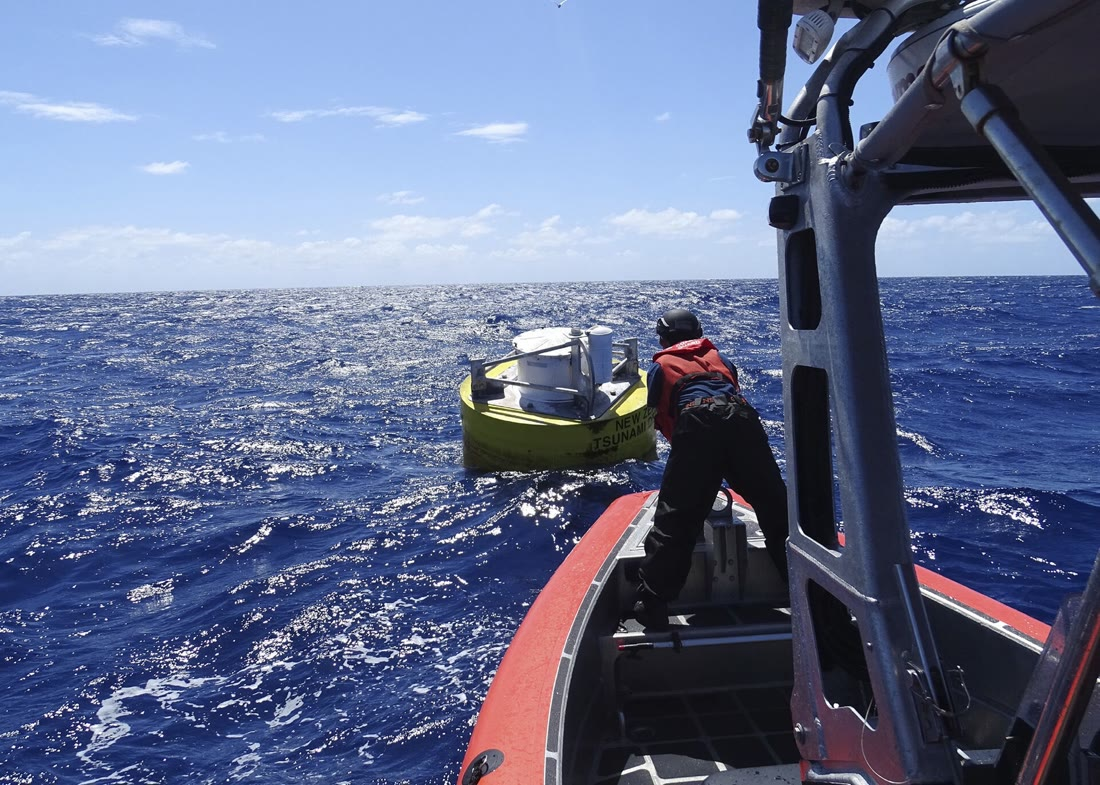
\includegraphics[width=\linewidth]{images/book1/g9-dart-buoy.jpg}
\end{minipage}\hfill
\begin{minipage}[c]{0.56\linewidth}\raggedright
{\small Seorang awak kapal Penjaga Pantai Amerika Serikat memeriksa
pelampung peringatan \omterm{def:g7:earthquakes:tsunami}{tsunami} di \omterm{def:g2:water-on-earth:ocean}{Samudra} Pasifik, pada bulan November
2021. Pelampung itu mengapung di atas perekam tekanan di dasar \omterm{def:g2:water-on-earth:ocean}{laut},
ribuan meter di bawahnya. U.S. Coast Guard (domain publik, melalui
Wikimedia Commons).}
\end{minipage}
% ledger: commons:dart-buoy
\label{fig:g9:natural-risks:buoy}
\end{omfigure}

\begin{history}[Jaringan pelampung]
Pada tahun 2001, deretan pertama yang terdiri atas enam stasiun semacam
itu selesai dipasang, di \omterm{def:g2:water-on-earth:ocean}{Samudra} Pasifik. Setelah \omterm{def:g7:earthquakes:tsunami}{tsunami} bulan Desember
2004, yang mencapai pantai-pantai \omterm{def:g2:water-on-earth:ocean}{Samudra} Hindia tanpa adanya sistem
peringatan (\cref{ch:g7:earthquakes}), jaringan itu berkembang: pada bulan
Maret 2008, sudah ada 39 stasiun.
\end{history}
% ledger: ndbc:dart

Peringatan hanya menyelamatkan nyawa jika sampai kepada orang-orang yang
tahu apa yang harus dilakukan dengannya: jalur ke tempat yang lebih tinggi
diberi rambu dan dilatih, tas siaga bencana sudah siap, sekolah-sekolah
mengadakan latihan. Di Armero, bahayanya sudah diketahui dan \omterm{def:g2:drawing-to-map:map}{petanya}
sudah digambar; peringatan itu tidak pernah sampai ke kota.
% ledger: ready:kit, usgs:armero

\section{Latihan}

\begin{exercise}[$\star$]\label{exo:g9:natural-risks:1}
Bahaya atau \omterm{def:g9:natural-risks:vulnerability}{kerentanan}? (a) \omterm{def:g1:landscapes-around-us:water}{Sungai} yang \omterm{def:g5:water-shapes-the-land:flood}{banjir} hampir setiap musim semi.
(b) Desa tanpa sistem peringatan. (c) Rumah-rumah bata yang berat tanpa
rangka. (d) Gempa kuat pada \omterm{def:g7:earthquakes:fault}{sesar} di dekatnya. (e) Kota yang dibangun di
mulut \omterm{def:g1:landscapes-around-us:landform}{lembah} yang dahulu pernah dilalui aliran lumpur.
\end{exercise}

\begin{exercise}[$\star$]\label{exo:g9:natural-risks:2}
Benar atau salah? Perbaiki kalimat yang salah. (a) \omterm{def:g5:natural-hazards:hazard}{Bahaya alam} di tempat
yang tidak berpenghuni merupakan \omterm{def:g9:natural-risks:risk}{risiko} tinggi. (b) \omterm{def:g9:natural-risks:prevention}{Pencegahan} dapat
menurunkan \omterm{def:g9:natural-risks:vulnerability}{kerentanan} sebuah kota. (c) \omterm{def:g9:natural-risks:hazard-map}{Peta bahaya} menunjukkan di mana
suatu bahaya dapat melanda. (d) Sistem peringatan yang baik membuat \omterm{def:g4:volcanoes-earthquakes-first-look:volcano}{gunung
api} kurang berbahaya.
\end{exercise}

\begin{exercise}[$\star$]\label{exo:g9:natural-risks:3}
Untuk setiap bahaya, katakan apakah bahaya itu dapat diprakirakan
beberapa hari atau beberapa jam sebelumnya: (a) \omterm{def:g5:natural-hazards:storm}{badai}; (b) \omterm{def:g5:water-shapes-the-land:flood}{banjir} setelah
\omterm{def:g4:clouds-rain-snow:precipitation}{hujan} lebat; (c) \omterm{def:g4:volcanoes-earthquakes-first-look:earthquake}{gempa bumi}; (d) tibanya \omterm{def:g7:earthquakes:tsunami}{tsunami} di pantai yang jauh dari
tempat asalnya.
\end{exercise}

\begin{exercise}[$\star$]\label{exo:g9:natural-risks:4}
% ledger: usgs:hvo-toolkit
Gunakan gambar \omterm{def:g4:volcanoes-earthquakes-first-look:volcano}{gunung api} yang diawasi. Apa yang diukur oleh setiap alat,
dan tanda peringatan \omterm{def:g4:volcanoes-earthquakes-first-look:eruption}{letusan} apa yang diawasinya? (a) \omterm{def:g7:earthquakes:seismometer}{Seismometer}.
(b) Tiltmeter. (c) Penerima GPS. (d) Alat ukur gas.
\end{exercise}

\begin{exercise}[$\star\star$]\label{exo:g9:natural-risks:5}
% ledger: usgs:armero
Pada tahun 1985, aliran lumpur Nevado del Ruiz mencapai Armero, yang
berjarak \qty{45}{km}, sekitar dua jam setelah \omterm{def:g4:volcanoes-earthquakes-first-look:eruption}{letusan}. (a) Berapa
kecepatan rata-ratanya, dalam kilometer per jam? (b) Orang berjalan kaki
dengan kecepatan sekitar \qty{4}{km/h}. Berapa jauh penduduk bisa
berjalan kaki dalam dua jam? (c) Mengapa mereka tidak pergi? (d) Berikan
dua hal yang dapat menyelamatkan mereka.
\end{exercise}

\begin{exercise}[$\star\star$]\label{exo:g9:natural-risks:6}
% ledger: (invented region: figdata/grade-9/flood_zone.py)
Gunakan \omterm{def:g2:drawing-to-map:map}{peta} zona \omterm{def:g5:water-shapes-the-land:flood}{banjir} Perbukitan Varden. (a) \omterm{def:g5:water-shapes-the-land:flood}{Banjir} mana yang
menggenangi jalur yang paling lebar? (b) Dengan kisi \omterm{def:g2:drawing-to-map:map}{peta}, ukurlah lebar
setiap zona melintasi \omterm{def:g1:landscapes-around-us:landform}{lembah} pada \qty{5}{km} ke timur. (c) Sebuah
lumbung berdiri di atas tanah \qty{6}{m} di atas \omterm{def:g1:landscapes-around-us:water}{sungai}. \omterm{def:g5:water-shapes-the-land:flood}{Banjir} mana di
antara ketiganya yang mencapainya? (d) Mengapa \omterm{def:g5:water-shapes-the-land:flood}{banjir} \qty{2}{m} di atas
\omterm{def:g1:landscapes-around-us:water}{sungai} adalah \omterm{def:g5:water-shapes-the-land:flood}{banjir} yang paling sering datang?
\end{exercise}

\begin{exercise}[$\star\star$]\label{exo:g9:natural-risks:7}
Tempatkan setiap keadaan pada kisi \omterm{def:g9:natural-risks:risk}{risiko} (bahaya rendah atau tinggi,
\omterm{def:g9:natural-risks:vulnerability}{kerentanan} rendah atau tinggi) dan katakan apakah \omterm{def:g9:natural-risks:risk}{risikonya} rendah,
sedang, atau tinggi. (a) Bangunan yang kokoh dan latihan rutin di kota
yang terletak pada \omterm{def:g7:earthquakes:fault}{sesar} aktif. (b) Bumi perkemahan di \omterm{def:g5:water-shapes-the-land:flood}{dataran banjir}
\omterm{def:g1:landscapes-around-us:water}{sungai} yang jarang \omterm{def:g5:water-shapes-the-land:flood}{banjir}. (c) Desa dengan rumah-rumah yang lemah di kaki
\omterm{def:g4:volcanoes-earthquakes-first-look:volcano}{gunung api} aktif, tanpa observatorium. (d) Kota di puncak \omterm{def:g1:landscapes-around-us:landform}{bukit} yang jauh
dari \omterm{def:g7:earthquakes:fault}{sesar}, \omterm{def:g1:landscapes-around-us:water}{sungai}, atau \omterm{def:g4:volcanoes-earthquakes-first-look:volcano}{gunung api} mana pun.
\end{exercise}

\begin{exercise}[$\star\star$]\label{exo:g9:natural-risks:8}
% ledger: iris:better-wall, explo:base-isolation
Tiga sekolah dibangun di atas tanah yang sama. Sekolah A adalah rangka
tiang dan balok dengan dinding bata di antaranya; sekolah B mempunyai
rangka yang sama dengan penguat diagonal dan dua dinding geser; sekolah C
mempunyai rangka sekolah B, yang berdiri di atas isolator. (a) Urutkan
ketiganya dari yang paling aman sampai yang paling tidak aman pada saat
gempa. (b) Jelaskan apa yang dilakukan penguat diagonal. (c) Jelaskan apa
yang dilakukan isolator.
\end{exercise}

\begin{exercise}[$\star\star$]\label{exo:g9:natural-risks:9}
% ledger: fema:flood-zones
Sebuah \omterm{def:g2:drawing-to-map:map}{peta} \omterm{def:g5:water-shapes-the-land:flood}{banjir} menunjukkan \omterm{def:g5:water-shapes-the-land:flood}{banjir} 100 tahunan, yang berpeluang 1 dari
100 untuk dicapai atau dilampaui dalam tahun mana pun. (a) Tuliskan
peluang ini sebagai persentase. (b) Seorang tetangga berkata, ``\omterm{def:g5:water-shapes-the-land:flood}{Banjir} 100
tahunan datang tahun lalu, jadi kita aman selama 99 tahun.'' Apa yang
salah? (c) Rata-rata, berapa banyak \omterm{def:g5:water-shapes-the-land:flood}{banjir} semacam itu yang akan datang
dalam 300 tahun?
\end{exercise}

\begin{exercise}[$\star\star$]\label{exo:g9:natural-risks:10}
% ledger: ndbc:dart, nws:tsunami-speed
Sebuah stasiun peringatan \omterm{def:g7:earthquakes:tsunami}{tsunami} membaca tekanan dasar \omterm{def:g2:water-on-earth:ocean}{laut} setiap
\qty{15}{s}. (a) Berapa kali pembacaan yang dilakukannya dalam satu jam?
(b) Dalam satu tahun yang terdiri atas 365 hari? Tuliskan jawabannya dalam
notasi ilmiah. (c) \omterm{def:g7:earthquakes:tsunami}{Tsunami} menyeberangi \omterm{def:g2:water-on-earth:ocean}{samudra} dalam dengan kecepatan
sekitar \qty{800}{km/h}. Berapa lama waktu yang diperlukannya untuk
mencapai pantai yang berjarak \qty{2400}{km}? (d) Mengapa waktu itu
penting?
\end{exercise}

\begin{exercise}[$\star\star\star$]\label{exo:g9:natural-risks:11}
% ledger: ready:kit
Sebuah keluarga beranggotakan empat orang menyiapkan tas siaga bencana
dengan air untuk 3 hari, sekitar \qty{3.8}{L} per orang per hari, untuk
minum dan membasuh diri. (a) Berapa liter air yang mereka perlukan?
(b) Berapa botol \qty{1.5}{L} jumlah itu? (c) Sebutkan empat barang lain
yang ada di dalam tas itu, dan katakan mengapa setiap barang berguna.
(d) Mengapa tas itu disimpan di dekat pintu?
\end{exercise}

\begin{exercise}[$\star\star\star$]\label{exo:g9:natural-risks:12}
% ledger: usgs:armero, usgs:hvo-toolkit
Sebuah kota terletak di tepi \omterm{def:g1:landscapes-around-us:water}{sungai}, di mulut \omterm{def:g1:landscapes-around-us:landform}{lembah} yang turun dari
\omterm{def:g4:volcanoes-earthquakes-first-look:volcano}{gunung api} yang puncaknya bersalju. Endapan aliran lumpur lama terdapat di
bawah jalan-jalannya. \omterm{def:g4:volcanoes-earthquakes-first-look:volcano}{Gunung api} itu mulai bergetar dengan gempa-gempa
kecil. Tulislah rencana \omterm{def:g9:natural-risks:prevention}{pencegahan} lima butir untuk kota itu. Untuk
setiap butir, katakan apakah butir itu bekerja pada sisi bahaya
(mengetahui dan mengawasi bahayanya) atau pada sisi \omterm{def:g9:natural-risks:vulnerability}{kerentanan} dari
\omterm{def:g9:natural-risks:risk}{risiko}.
\end{exercise}

\section{Soal: Di mana sekolah baru harus dibangun?}

\begin{problem}[{Soal akhir pekan --- sebuah sekolah baru ditempatkan pada
peta Perbukitan Varden, jauh dari banjir, lereng yang curam, dan sesar;
jawaban terakhirnya adalah banyaknya rumah di dalam zona banjir}]
\label{pb:g9:natural-risks:1}
% ledger: (invented region: figdata/grade-9/flood_zone.py: sites A, B, C; 17 of 28 houses in the 5 m zone)
Desa di Perbukitan Varden memerlukan sekolah baru, dan tiga lokasi
ditawarkan: A, B, dan C, pada \omterm{def:g2:drawing-to-map:map}{peta} di bawah. Zona \omterm{def:g5:water-shapes-the-land:flood}{banjir} yang berarsir
pada \omterm{def:g2:drawing-to-map:map}{peta} adalah semua tanah yang kurang dari \qty{5}{m} di atas \omterm{def:g1:landscapes-around-us:water}{sungai},
yang akan digenangi oleh \omterm{def:g5:water-shapes-the-land:flood}{banjir} besar. Tabel ini memberikan, untuk setiap
lokasi, \omterm{def:g4:world-physical-map:altitude}{ketinggian} tanah, ketinggian sungai di sampingnya, dan seberapa
tinggi tanah naik sepanjang \qty{200}{m} yang diukur mendatar melintasi
lereng.

\begin{center}
{\small
\begin{tabular}{|c|c|c|c|}
\hline
lokasi & \omterm{def:g4:world-physical-map:altitude}{ketinggian} tanah & ketinggian sungai di sampingnya & kenaikan tanah sepanjang \qty{200}{m} \\
\hline
A & \qty{137}{m} & \qty{137}{m} & \qty{1.4}{m} \\
B & \qty{276}{m} & \qty{126}{m} & \qty{83}{m} \\
C & \qty{236}{m} & \qty{143}{m} & \qty{20}{m} \\
\hline
\end{tabular}}
\end{center}

\begin{omfigure}
\begin{tikzpicture}
\begin{axis}[axis equal image, xmin=3.5, xmax=7, ymin=2.7, ymax=5.5, width=11.5cm,
  enlargelimits=false, tick label style={font=\scriptsize}, xlabel={timur (km)},
  ylabel={utara (km)}, label style={font=\small}, xtick={3.5,4,...,7}, ytick={3,3.5,...,5.5}]
\addplot[contour] table {figdata/out/grade-9-flood_zone-contours.dat};
\addplot[index contour] table {figdata/out/grade-9-flood_zone-index.dat};
\addplot[fill=blue!25, draw=blue!50, line width=0.3pt] table {figdata/out/grade-9-flood_zone-zone.dat} -- cycle;
\addplot[only marks, mark=none, point meta=explicit symbolic, nodes near coords,
  nodes near coords align={center}, nodes near coords style={font=\tiny, fill=white, inner sep=0.6pt, text=omContour}]
  table[meta=z] {figdata/out/grade-9-flood_zone-index-lab.dat};
\addplot[river] table {figdata/out/grade-9-flood_zone-river.dat};
\addplot[fault] table {figdata/out/shared-region-fault.dat};
\addplot[only marks, mark=square*, mark size=1.5pt, mark options={fill=black}] table {figdata/out/grade-9-flood_zone-houses-in.dat};
\addplot[only marks, mark=square*, mark size=1.5pt, mark options={fill=black}] table {figdata/out/grade-9-flood_zone-houses-out.dat};
\addplot[only marks, mark=*, mark size=2.6pt, mark options={fill=omWarm, draw=black}, point meta=explicit symbolic,
  nodes near coords, nodes near coords align={anchor=south west},
  nodes near coords style={font=\small\bfseries, fill=white, inner sep=1pt, xshift=2.5pt, yshift=2.5pt}]
  table[meta=name] {figdata/out/grade-9-flood_zone-sites.dat};
\node[font=\footnotesize, fill=white, inner sep=1pt, anchor=west] at (axis cs:6.42,5.05) {sesar};
\coordinate (na) at (axis cs:3.7,4.75);
\fill[black] (axis cs:5.8,2.85) rectangle (axis cs:5.925,2.9);
\fill[white] (axis cs:5.925,2.85) rectangle (axis cs:6.05,2.9);
\fill[black] (axis cs:6.05,2.85) rectangle (axis cs:6.175,2.9);
\fill[white] (axis cs:6.175,2.85) rectangle (axis cs:6.3,2.9);
\draw[black, line width=0.4pt] (axis cs:5.8,2.85) rectangle (axis cs:6.3,2.9);
\node[font=\footnotesize, above, inner sep=1.5pt, fill=white] at (axis cs:6.05,2.9) {\qty{500}{m}};
\end{axis}
\fill[white, opacity=0.85] ($(na)+(-0.35,-0.1)$) rectangle ($(na)+(0.35,1.45)$);
\pic at (na) {northarrow};
\end{tikzpicture}

{\small Desa, ketiga lokasi sekolah, dan zona \omterm{def:g5:water-shapes-the-land:flood}{banjir} (berarsir), pada \omterm{def:g2:drawing-to-map:map}{peta}
Perbukitan Varden (garis-garis tipis yang sama tingginya setiap
\qty{10}{m}). Setiap persegi kecil berwarna hitam adalah sebuah rumah.
Garis hitam yang tebal adalah sebuah \omterm{def:g7:earthquakes:fault}{sesar}.}
\label{fig:g9:natural-risks:school-map}
\end{omfigure}

\noindent\textbf{Bagian I --- Zona banjir.}\par\nopagebreak
\begin{enumerate}[beginpenalty=10000]
  \item Dengan memakai ketinggian sungai dalam tabel, katakan ke arah mana
        \omterm{def:g1:landscapes-around-us:water}{sungai} itu mengalir.
  \item Hitunglah \omterm{def:g4:world-physical-map:altitude}{ketinggian} setiap lokasi di atas \omterm{def:g1:landscapes-around-us:water}{sungai} di sampingnya.
  \item Lokasi mana di antara ketiganya yang terletak di zona \omterm{def:g5:water-shapes-the-land:flood}{banjir}?
  \item Gunakan batang \omterm{def:g2:drawing-to-map:scale}{skala} untuk mengukur lebar zona \omterm{def:g5:water-shapes-the-land:flood}{banjir}, melintasi
        \omterm{def:g1:landscapes-around-us:landform}{lembah}, di lokasi A.
\end{enumerate}

\noindent\textbf{Bagian II --- Lereng dan sesar.}\par\nopagebreak
\begin{enumerate}[resume, beginpenalty=10000]
  \item Kemiringan lereng dalam persen adalah kenaikan tanah untuk setiap
        \qty{100}{m} yang diukur mendatar. Hitunglah kemiringan lereng di
        setiap lokasi.
  \item Lokasi mana yang akan terancam \omterm{def:g5:natural-hazards:landslide}{tanah longsor}? Jelaskan.
  \item Gunakan batang \omterm{def:g2:drawing-to-map:scale}{skala} untuk memperkirakan jarak dari setiap lokasi
        ke \omterm{def:g7:earthquakes:fault}{sesar}.
  \item Misalkan \omterm{def:g7:earthquakes:fault}{sesar} itu masih dapat bergerak. Mengapa tanah tepat di
        atasnya merupakan tempat yang buruk untuk sekolah?
\end{enumerate}

\noindent\textbf{Bagian III --- Memilih.}\par\nopagebreak
\begin{enumerate}[resume, beginpenalty=10000]
  \item Buatlah tabel dengan satu baris untuk setiap lokasi dan tiga kolom:
        di zona \omterm{def:g5:water-shapes-the-land:flood}{banjir}? lereng curam? di atas \omterm{def:g7:earthquakes:fault}{sesar}? Isilah dengan ya atau
        tidak.
  \item Lokasi mana yang akan kamu pilih? Berikan alasan pilihanmu dengan
        memakai tabel itu.
  \item Lokasi yang dipilih tetap berada di wilayah yang tanahnya dapat
        berguncang. Sebutkan dua cara membangun sekolah itu, dan satu
        kebiasaan murid-muridnya, yang menurunkan \omterm{def:g9:natural-risks:vulnerability}{kerentanannya}.
  \item Sekolah itu juga akan menjadi tempat pengungsian selama \omterm{def:g5:water-shapes-the-land:flood}{banjir}.
        Hitunglah rumah-rumah di desa itu yang berdiri di dalam zona \omterm{def:g5:water-shapes-the-land:flood}{banjir}.
        Berapa bagian dari seluruh rumah itu?
\end{enumerate}
\end{problem}
